\documentclass[11pt]{article}
\usepackage[margin=1in]{geometry}
\usepackage{booktabs}
\usepackage{longtable}
\usepackage{graphicx}
\usepackage{hyperref}
\usepackage{xcolor}

\title{Reproducing LEBench on a Virtual Machine\\
\large An Analysis of Performance Evolution of Linux's Core Operations}
\author{Haoyu Zou \quad 5260000157\\
CS340 Operating Systems, 2026--2027}
\date{3 November 2026}

\begin{document}
\maketitle

\section{Introduction and claims}

Ren et al.\ measured the latency of Linux core operations from 3.0 through 4.20 and argued that the kernel got slower, mostly because of security work, new features, and a few configuration mistakes \cite{ren2019lebench}. The operations are the ones LEBench times directly: \texttt{getpid}, context switch, fork, read/write, mmap/munmap, page fault, send/recv, and select/poll/epoll.

Three claims are tied to the paper:

\begin{enumerate}
\item \textbf{Figure 1(a).} Relative to Linux 4.0, later kernels are slower on these operations, except big write and big munmap. Most tests are also slower than on 3.0, and many are at least 50\% slower.
\item \textbf{Table 3 and Figure 2.} Eleven changes explain the large jumps. Four are security patches, four are features, and three are configuration mistakes.
\item \textbf{Section 5.} Turning those eleven changes off speeds Redis, Apache, and Nginx by up to 56\%, 33\%, and 34\%.
\end{enumerate}

This reproduction tests claim 1 on the kernel list shipped with the authors' experiment notes, and tests one factor from claim 2 (page-table isolation) as the extension. Claim 3 is not run. The authors' \texttt{EXPERIMENTS.md} lists 41 Ubuntu mainline builds, from 3.0.7 to 4.20.13. The paper text says 36 versions. The driver attempts every release in that file.

\section{Reproduction setup}

\subsection{Starting code}

The benchmark is the authors' LEBench tree at commit \texttt{6aa7801} (\url{https://github.com/LinuxPerfStudy/LEBench}), Apache-2.0, copyright 2019 University of Toronto. \texttt{TEST\_DIR/OS\_Eval.c}, \texttt{run.py}, and \texttt{get\_kern.py} are unchanged. The course runner is \texttt{course/OS\_Eval\_reduced.c}, generated from that file by \texttt{course/make\_reduced\_eval.py}. It keeps the same \texttt{clock\_gettime} intervals and the same K-best rule (five samples within 5\%). \texttt{BASE\_ITER} is 40 instead of 10{,}000, the 60-second settle is omitted, and three cases that either block or dominate runtime are compiled out: the 96\,KB send/recv pair, the 12{,}000-page fork, and the 10{,}000-page file tests. A null K-best result, which aborts the original program on a noisy virtual machine, falls back to the smallest sample.

A separate rewrite that reimplemented the tests with \texttt{rdtsc} was not used. Section~\ref{sec:rewrite} says why.

\subsection{Environment}

\begin{center}
\begin{tabular}{@{}ll@{}}
\toprule
Item & Setting \\
\midrule
Host & Windows 11, 13th Gen Intel Core i7-13700H \\
Hypervisor & VirtualBox 7.2.22, legacy BIOS, NAT \\
Guest & Ubuntu 16.04.6 LTS, English \\
Resources & 2 virtual CPUs, 4\,GB RAM, 80\,GB disk on \texttt{D:} \\
Compiler & gcc 5.4.0 (\texttt{-O0 -pthread}, the upstream makefile flags) \\
Known-good kernel & 4.4.0-210-generic, used only to install and recover \\
\bottomrule
\end{tabular}
\end{center}

Memory integrity is enabled on the host, so VirtualBox cannot use its fast hypervisor path. The guest CPU model string is still the host's i7-13700H. That CPU reports Meltdown as ``Not affected''.

\subsection{Workloads}

Each booted kernel runs \texttt{course/sweep\_bench} three times as root. The binary is the reduced \texttt{OS\_Eval}. It writes the authors' CSV: one K-best row and one average row per test, in seconds. The reported number is the mean and sample standard deviation of the three K-best values. Logs are \texttt{results/kernels/<release>/runN.csv} plus stdout, stderr, the exit code, and \texttt{environment.txt}.

Kernel packages come from the authors' backup, \url{https://github.com/LinuxPerfStudy/ExperimentSetup}, directory \texttt{default\_ubuntu\_kernels}. The driver downloads the \texttt{linux-image} deb (the \texttt{unsigned} package where that is the only image), installs it, and selects it for one boot with \texttt{grub-reboot}. A panic returns to 4.4.0-210 on the next power-on. It does not run the upstream \texttt{grub-install} against a partition.

\subsection{Deviations}

\begin{center}
\small
\begin{tabular}{@{}p{0.22\linewidth}p{0.24\linewidth}p{0.22\linewidth}p{0.22\linewidth}@{}}
\toprule
Item & Paper & Used here & Reason \\
\midrule
Machine & HP DL160 G9, Xeon E5-2630 v3, 128\,GB, SSD & VirtualBox on an i7-13700H, 2 vCPU, 4\,GB & The server is not available. Comparisons stay on one guest. \\
Kernel count & 36 versions in the paper text & All 41 releases listed by the authors & The released list is the reproducible set. \\
Iterations & \texttt{BASE\_ITER} 10{,}000 and a 60\,s settle & \texttt{BASE\_ITER} 40, no settle & A full pass is hours per kernel on this guest. The K-best rule is unchanged. \\
Omitted tests & 96\,KB send/recv, 12{,}000-page fork, 10{,}000-page I/O & Not compiled in & The upstream comment says the large send blocks on old kernels. The other two dominate runtime. \\
Statistics & K-best inside one process & That value, then mean $\pm$ sample standard deviation over 3 processes & The course requires the cross-run statistic. \\
Applications & Redis, Apache, Nginx & Not run & Claim 1 and one security switch come first. \\
\bottomrule
\end{tabular}
\end{center}

\section{Results}

\subsection{Page-table isolation on the installed kernel}
\label{sec:ext}

This comparison changes one factor. Kernel 4.4.0-210-generic is booted twice: the default command line, and the same kernel with \texttt{nopti}. Hardware, binary, and iteration count stay the same. \texttt{/sys/devices/system/cpu/vulnerabilities/meltdown} reads ``Not affected'' in both boots. Spectre v2 stays on Enhanced IBRS.

Table~\ref{tab:nopti} is computed by \texttt{scripts/render\_results.py} from \texttt{results/kernel\_summary.csv}. ``Overlap'' means the two mean$\pm$stdev intervals touch.

\begin{table}[ht]
\centering
\caption{Same kernel and binary, default command line versus \texttt{nopti}. Three runs each.}
\label{tab:nopti}
\begin{tabular}{@{}lrrrr@{}}
\toprule
Test & Default & $nopti$ & Change & Intervals overlap? \\
\midrule
getpid & 314 ns & 295 ns & -6\% & yes \\
context siwtch & 11.2 us & 12.9 us & +15\% & yes \\
send & 600 ns & 693 ns & +15\% & yes \\
recv & 692 ns & 764 ns & +10\% & yes \\
fork & 92.8 us & 254.0 us & +174\% & no \\
small read & 784 ns & 946 ns & +21\% & yes \\
small write & 1.9 us & 2.0 us & +7\% & yes \\
big write & 1.66 ms & 3.62 ms & +118\% & yes \\
big munmap & 269.5 us & 266.3 us & -1\% & yes \\
select & 1.2 us & 1.5 us & +29\% & yes \\
poll & 847 ns & 1.1 us & +26\% & yes \\
epoll & 905 ns & 1.0 us & +12\% & yes \\
\bottomrule
\end{tabular}

\end{table}

Fast operations move by less than their run-to-run spread. \texttt{fork} is slower with \texttt{nopti}, and the intervals do not overlap. That is the opposite of the paper's KPTI tax, and it is not a clean ablation: this CPU does not enable Meltdown page-table isolation in the first place.

\subsection{Kernel sweep}

Of the 41 releases in \texttt{EXPERIMENTS.md}, 34 booted far enough for three runs. Kernels 3.0.7 through 3.5.4 install and then never answer sshd; they are listed in \texttt{results/kernels/boot-failures.txt} and have no latency. Linux 4.19.11 needs a \texttt{linux-modules} package that is no longer published at the Ubuntu mainline URL used for 4.16, 4.17, 4.18, and 4.20, so that one release was not installed. The 4.4.0-210 pair is the guest's recovery kernel and is not one of the 41.

Across 627 later-kernel measurements, 271 (43\%) have a higher mean than the same test on 4.0.5 and 76 (12\%) have a mean at least 50\% higher. 117 of those measurements have non-overlapping mean$\pm$stdev intervals and a higher mean, which is the bar used in the analysis.


\begin{table}[ht]
\centering
\caption{Paper versus this guest. The metric is the sign of the latency change from Linux 4.0, which is what Figure 1(a) plots.}
\label{tab:paper}
\begin{tabular}{@{}p{0.22\linewidth}p{0.36\linewidth}p{0.34\linewidth}@{}}
\toprule
Item & Paper & Ours \\
\midrule
Later kernels vs 4.0 & Most tests slower, and many by at least 50\% & 271 of 627 means (43\%) are higher; 76 (12\%) are at least 50\% higher \\
vs Linux 3.0 & 75\% of tests slower & No measurement: 3.0.7--3.5.4 never reached sshd \\
\bottomrule
\end{tabular}
\end{table}

Those 627 rows are every test on the 19 kernels newer than 4.0.5 that finished three runs. A zero K-best on 3.6.10 (getpid and a few other tests) is a failed window: the average in the same CSV is not zero, and 3.6.10 is not the baseline, so it is not in the 627. Table~\ref{tab:kernels} shows three tests. Every mean is the mean of three K-best values in \texttt{results/kernels/<release>/run\{1,2,3\}.csv}, and the full set is \texttt{results/kernel\_summary.csv}.

{\small
\begin{longtable}{@{}lrrr@{}}
\caption{Mean $\pm$ sample standard deviation of three K-best runs.}\label{tab:kernels}\\
\toprule
Kernel & getpid & big write & big munmap \\
\midrule
\endfirsthead
\toprule
Kernel & getpid & big write & big munmap \\
\midrule
\endhead
\bottomrule
\endfoot
3.6.10 & 0$\pm$0 ns & 1.42$\pm$0.12 ms & 220.4$\pm$190.9 us \\
3.7.9 & 422$\pm$61 ns & 2.63$\pm$1.18 ms & 273.1$\pm$6.7 us \\
3.8.10 & 317$\pm$44 ns & 1.91$\pm$0.44 ms & 403.2$\pm$168.1 us \\
3.9.8 & 295$\pm$18 ns & 2.70$\pm$1.34 ms & 459.6$\pm$272.4 us \\
3.10.10 & 921$\pm$23 ns & 2.26$\pm$0.24 ms & 329.0$\pm$50.8 us \\
3.11.6 & 325$\pm$43 ns & 2.04$\pm$0.42 ms & 379.1$\pm$58.3 us \\
3.12.8 & 1.0$\pm$0.1 us & 2.65$\pm$1.66 ms & 350.1$\pm$61.8 us \\
3.13.7 & 1.1$\pm$0.2 us & 1.63$\pm$0.07 ms & 321.0$\pm$10.7 us \\
3.14.6 & 878$\pm$26 ns & 2.32$\pm$0.15 ms & 373.3$\pm$48.1 us \\
3.15.8 & 998$\pm$126 ns & 2.38$\pm$0.56 ms & 340.3$\pm$87.3 us \\
3.16.3 & 322$\pm$41 ns & 1.09$\pm$0.46 ms & 178.7$\pm$83.5 us \\
3.17.6 & 238$\pm$75 ns & 1.54$\pm$0.68 ms & 218.6$\pm$8.5 us \\
3.18.6 & 293$\pm$37 ns & 2.93$\pm$1.42 ms & 228.9$\pm$29.7 us \\
3.19.3 & 253$\pm$6 ns & 2.08$\pm$0.40 ms & 200.3$\pm$0.5 us \\
4.0.5 & 245$\pm$0 ns & 1.66$\pm$0.28 ms & 199.7$\pm$3.5 us \\
4.1.6 & 255$\pm$6 ns & 1.95$\pm$0.50 ms & 193.6$\pm$8.1 us \\
4.2.5 & 248$\pm$9 ns & 1.37$\pm$0.57 ms & 161.7$\pm$55.2 us \\
4.3.3 & 224$\pm$93 ns & 1.67$\pm$0.55 ms & 157.4$\pm$54.9 us \\
4.4.5 & 238$\pm$8 ns & 1.65$\pm$0.10 ms & 198.6$\pm$5.9 us \\
4.5.4 & 189$\pm$0 ns & 1.59$\pm$0.15 ms & 166.4$\pm$50.7 us \\
4.6.4 & 117$\pm$62 ns & 1.67$\pm$0.94 ms & 184.9$\pm$87.7 us \\
4.7.6 & 192$\pm$1 ns & 4.24$\pm$2.97 ms & 334.2$\pm$100.0 us \\
4.8.14 & 225$\pm$29 ns & 2.87$\pm$1.62 ms & 210.6$\pm$0.5 us \\
4.9.11 & 203$\pm$85 ns & 3.72$\pm$1.20 ms & 480.8$\pm$415.3 us \\
4.10.13 & 197$\pm$6 ns & 1.71$\pm$0.15 ms & 206.9$\pm$3.8 us \\
4.11.8 & 212$\pm$28 ns & 1.63$\pm$0.40 ms & 335.8$\pm$236.1 us \\
4.12.10 & 195$\pm$9 ns & 1.58$\pm$0.27 ms & 247.3$\pm$58.3 us \\
4.13.12 & 251$\pm$10 ns & 1.90$\pm$0.73 ms & 211.4$\pm$2.6 us \\
4.14.15 & 535$\pm$12 ns & 1.77$\pm$0.21 ms & 206.0$\pm$6.4 us \\
4.15.15 & 248$\pm$30 ns & 2.55$\pm$0.64 ms & 212.3$\pm$39.9 us \\
4.16.13 & 100$\pm$0 ns & 657.6$\pm$46.5 us & 83.6$\pm$0.8 us \\
4.17.14 & 100$\pm$1 ns & 611.1$\pm$12.2 us & 84.0$\pm$1.0 us \\
4.18.16 & 100$\pm$0 ns & 671.0$\pm$17.4 us & 79.5$\pm$0.7 us \\
4.20.13 & 230$\pm$44 ns & 2.27$\pm$0.47 ms & 192.7$\pm$3.9 us \\
\end{longtable}

}

\IfFileExists{generated/relative_latency.pdf}{%
\begin{figure}[ht]
\centering
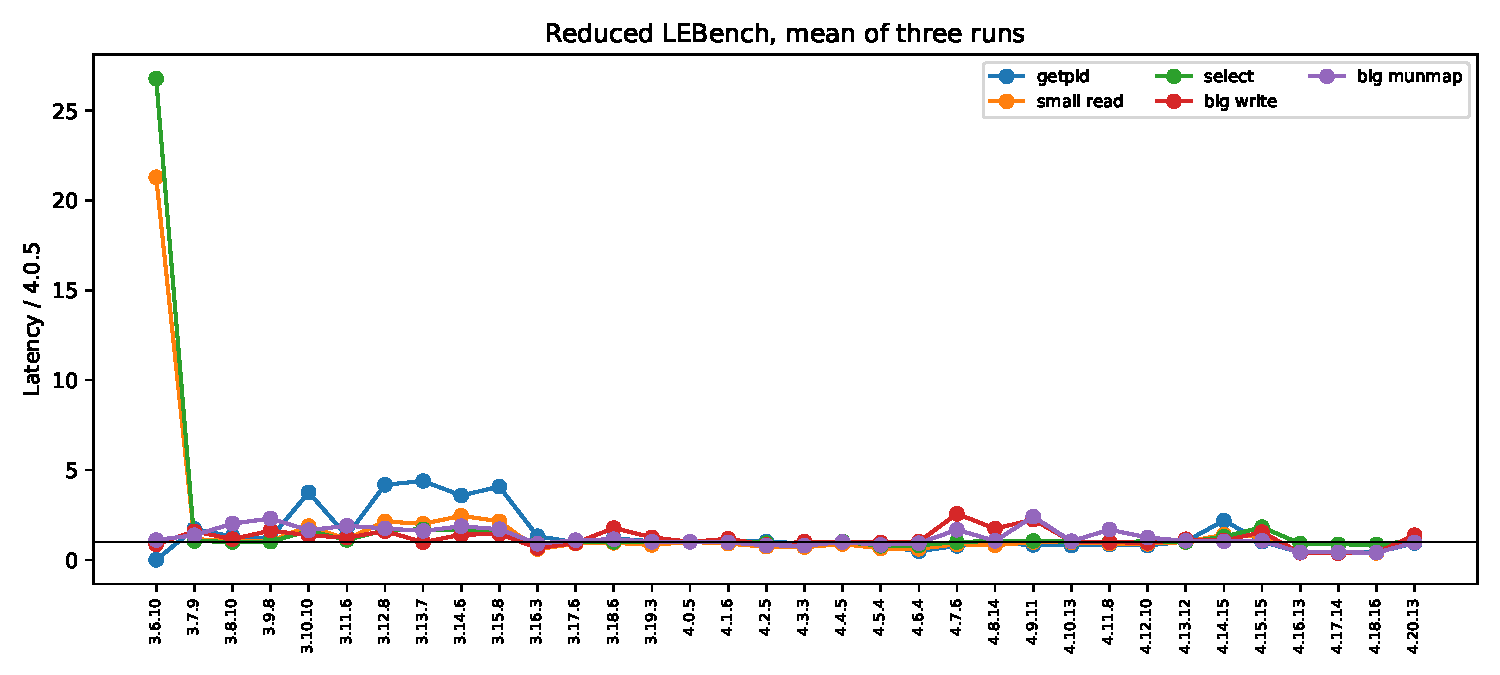
\includegraphics[width=\linewidth]{generated/relative_latency.pdf}
\caption{Latency divided by the 4.0.5 result on this guest. The line at 1 is the paper's baseline kernel.}
\label{fig:rel}
\end{figure}
}{}

\section{Analysis}

Claim 1 is about the sign of the change from 4.0, not the absolute nanoseconds. Absolute times here are not the paper's times: the guest has two slow virtual CPUs, the disk is a virtual disk, and the iteration count is shorter, so a single outlier moves the K-best window. The standard deviations in Table~\ref{tab:nopti} are often a large fraction of the mean. A difference smaller than the standard deviation is not evidence. The verdict below uses that rule: a later kernel counts as slower only when its mean$\pm$stdev interval sits entirely above the 4.0.5 interval.

On that rule, claim 1 is \textbf{not supported} on this guest. Only 271 of 627 later-kernel measurements (43\%) even have a higher mean than 4.0.5, and only 117 have a non-overlapping interval and a higher mean. The paper's ``most tests are slower, and many by at least 50\%'' does not describe this table: 76 of 627 (12\%) have a mean at least 50\% higher. Broken out for the 19 later kernels, getpid has a higher mean on 5 and a clearly faster interval on 9; fork has a higher mean on 0. Big write, which the paper treats as an exception that got faster, has a higher mean on 11 of 19 kernels, but only 1 of those intervals clears the noise. The comparison with Linux 3.0 is \textbf{inconclusive}: 3.0.7 through 3.5.4 never reached sshd, so there is no 3.0 baseline on this guest.

Claim 2 is only touched by the \texttt{nopti} switch. The paper's KPTI result needs a CPU that pays for page-table isolation. The i7-13700H reports that it does not. The switch still changes \texttt{fork}, so the command line is not a no-op, but it does not reproduce ``KPTI makes \texttt{getpid}, read, and recv slower.'' That part of claim 2 is \textbf{not supported} here.

Claim 3 is not tested. There is no Redis, Apache, or Nginx number in this repository, so the application claim is \textbf{inconclusive}.

What this run cannot show is the heatmap on the original server, the eleven-way ablation, or the application speedups. Kernels that do not reach sshd are recorded as boot failures in \texttt{results/kernels/progress.log} and are not given a latency.

\section{Extension}
\label{sec:batch}

The reduced suite times one \texttt{getpid} between two \texttt{clock\_gettime} calls. On 4.0.5 that empty pair, the \texttt{ref} row, is 156 $\pm$ 64 ns, and the \texttt{getpid} row is 245 $\pm$ 0 ns, so the timer is a large part of the number. The extension changes only that test. \texttt{course/OS\_Eval\_batched.c} is the reduced source with \texttt{getpid} rewritten to time 1{,}000 calls and divide by 1{,}000. K-best, \texttt{BASE\_ITER}, the compiler flags, and every other test stay the same. Each kernel ran the new binary three times. Logs are \texttt{results/batching/<release>/run\{1,2,3\}.csv}.

\begin{table}[ht]
\centering
\caption{Mean $\pm$ sample standard deviation of three K-best runs. Single-shot numbers are the reduced sweep; batched numbers are the one-line change above.}
\label{tab:batch}
\begin{tabular}{@{}lrr@{}}
\toprule
Kernel & Single-shot getpid & Batched getpid \\
\midrule
4.0.5 & 245 $\pm$ 0 ns & 129 $\pm$ 0 ns \\
4.4.0-210 & 314 $\pm$ 39 ns & 127 $\pm$ 40 ns \\
\bottomrule
\end{tabular}

\end{table}

On 4.0.5 the batched per-call cost is 129 ns, against 245 ns for one call. The two intervals do not overlap. The same binary's empty clock pair that day was 132 $\pm$ 19 ns, close to the batched per-call figure, which is what a timer-dominated sample looks like. On 4.4.0-210 the single-shot mean is 314 ns and its interval sits entirely above 4.0.5. After batching, the means are 127 ns and 129 ns, and the intervals overlap. The apparent \texttt{getpid} slowdown between these two kernels does not survive the change. \texttt{small read} on the batched binary stays within the single-shot spread (4.0.5: 813 $\pm$ 72 ns against 726 $\pm$ 73 ns), so the rest of the suite did not move with this edit.

\section{The other implementation}
\label{sec:rewrite}

A second tree, written as a from-scratch LEBench, lives outside this repository. It is a Linux C program (\texttt{src/bench\_*.c}) plus a Chinese report whose result table is empty. It was not used for the numbers above. The useful ideas in it are the K-best description and the list of operations. The measurement itself should not be substituted for \texttt{OS\_Eval}:

\begin{itemize}
\item It times with \texttt{rdtsc} and does not serialize the instruction stream. On this VirtualBox guest the TSC is not a stable offset from the host, which is why the authors' code uses \texttt{clock\_gettime}.
\item \texttt{select} allocates and fills the descriptor bitmap inside the timed region, so the number includes allocator traffic.
\item Context switch is one long loop divided by the iteration count. That is an average, not the paper's K-best of repeated trials, and it never raises the priority to $-20$.
\item The page-fault sample touches every page and divides by the page count. Fault-around fills neighboring pages on the first miss, so later touches in that sample are often not faults. \texttt{OS\_Eval} times one touch.
\item Iteration counts, the empty-syscall choice, and the lack of a third process run all differ from the paper and from the course rule.
\item It was checked by compiling against stand-in headers on Windows. It had not been executed on Linux, and the report says so.
\end{itemize}

The changes that make the course tree more faithful are the ones in \texttt{course/} and \texttt{scripts/vm\_kernel\_sweep.py}: call the authors' functions, keep K-best, repeat three times, create the Unix-socket directory \texttt{OS\_Eval} concatenates onto \texttt{LEBENCH\_DIR}, and boot with \texttt{grub-reboot} instead of installing GRUB onto a partition.

\section{Conclusion}

The reproduction is partial. Thirty-four of the 41 listed kernels ran the reduced benchmark three times. On those logs, the claim that most core operations got slower after 4.0 is not supported, and the \texttt{nopti} switch does not reproduce the KPTI slowdown on a CPU that is not subject to Meltdown. Batching \texttt{getpid} on 4.0.5 and 4.4.0-210 cuts the reported per-call cost by about half and removes the slowdown between those two kernels, so that one row was mostly the timer. The application section and the eleven-cause ablation are not reproduced. The practical lesson is that a microbenchmark copied onto a new timer, and a kernel image that does not boot, both fail quietly: the first still prints a number, and the second never gets far enough to print one. The logs have to show which of those happened.

\section*{Contribution statement}

Haoyu Zou (5260000157) imported LEBench at \texttt{6aa7801}, built the Ubuntu 16.04.6 guest, wrote the reduced runner and the reboot driver, collected the logs under \texttt{results/kernels/}, measured the batched-\texttt{getpid} variant under \texttt{results/batching/}, and wrote this report and the slides. Commits for this work use that student ID and name.

\section*{AI usage statement}

An AI coding assistant in Cursor drafted the runner, the reboot script, this report, and the slides, and operated the virtual machine. Kernel packages, the benchmark source, and the latency numbers are from the LEBench authors and from the guest logs. The assistant did not invent measurements.

\begin{thebibliography}{9}
\bibitem{ren2019lebench}
Xiang (Jenny) Ren, Kirk Rodrigues, Luyuan Chen, Camilo Vega, Michael Stumm, and Ding Yuan.
An Analysis of Performance Evolution of Linux's Core Operations.
In \emph{Proceedings of SOSP}, 2019.
\url{https://doi.org/10.1145/3341301.3359640}
\end{thebibliography}

\end{document}
